\documentclass{standalone}

\usepackage{tikz}
\usetikzlibrary{decorations.markings}

\usepackage{amsmath}

\begin{document}

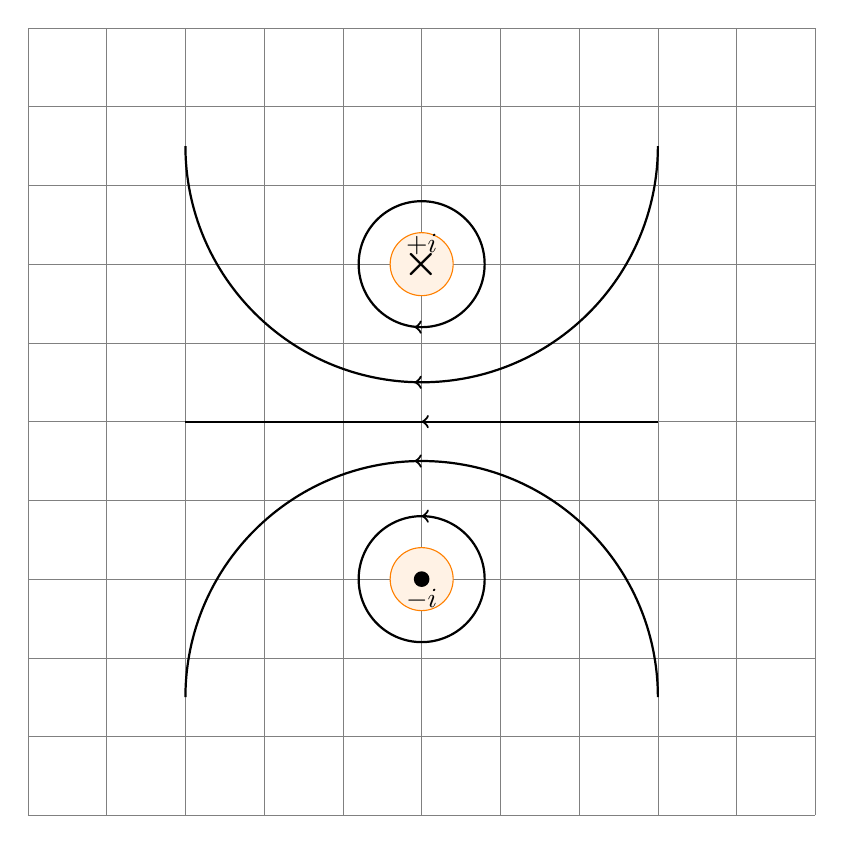
\begin{tikzpicture}

\draw[help lines] grid (10,10);

%position of bottom wire
\coordinate (A1) at (5,3);

%position of top wire
\coordinate (A2) at (5,7);

%point defining the top-most mag. field line
\coordinate (start) at (8,10);
\coordinate (through) at (5,6);
\coordinate (end) at (2,10);


% node with negative charge
\draw[fill=orange!10, draw=orange] (A1) circle[radius=0.4] node[anchor=north] {$-i$};
\node[circle, fill=black, inner sep=2pt]  at (A1) {};

% node with positive charge
\draw[fill=orange!10, draw=orange] (A2) circle[radius=0.4] node[anchor=south] {$+i$};
\node at (A2) {\Large$\boldsymbol{\times}$};

% magnetic field lines
\draw[thick, postaction={decorate}, decoration={markings, mark=at position 0.5 with {\arrow{<}}}] (2,8.5) arc (-180:0:3cm and 3cm);
\draw[thick, postaction={decorate}, decoration={markings, mark=at position 0.75 with {\arrow{<}}}] (5,7) circle[radius=0.8];
\draw[thick, postaction={decorate}, decoration={markings, mark=at position 0.5 with {\arrow{>}}}] (8,5) -- (2,5);
\draw[thick, postaction={decorate}, decoration={markings, mark=at position 0.5 with {\arrow{<}}}] (2,1.5) arc (180:0:3cm and 3cm);
\draw[thick, postaction={decorate}, decoration={markings, mark=at position 0.25 with {\arrow{>}}}] (5,3) circle[radius=0.8];


\end{tikzpicture}

\end{document}